\chapter{Resultados}
Neste capítulo são demonstrados os resultados obtidos após o desenvolvimento do projeto.
\section{Sistema completo}

 O sistema completado é demonstrado na Figura \ref{fig:luvaMontada}.

\begin{figure}[H]
	\centering
	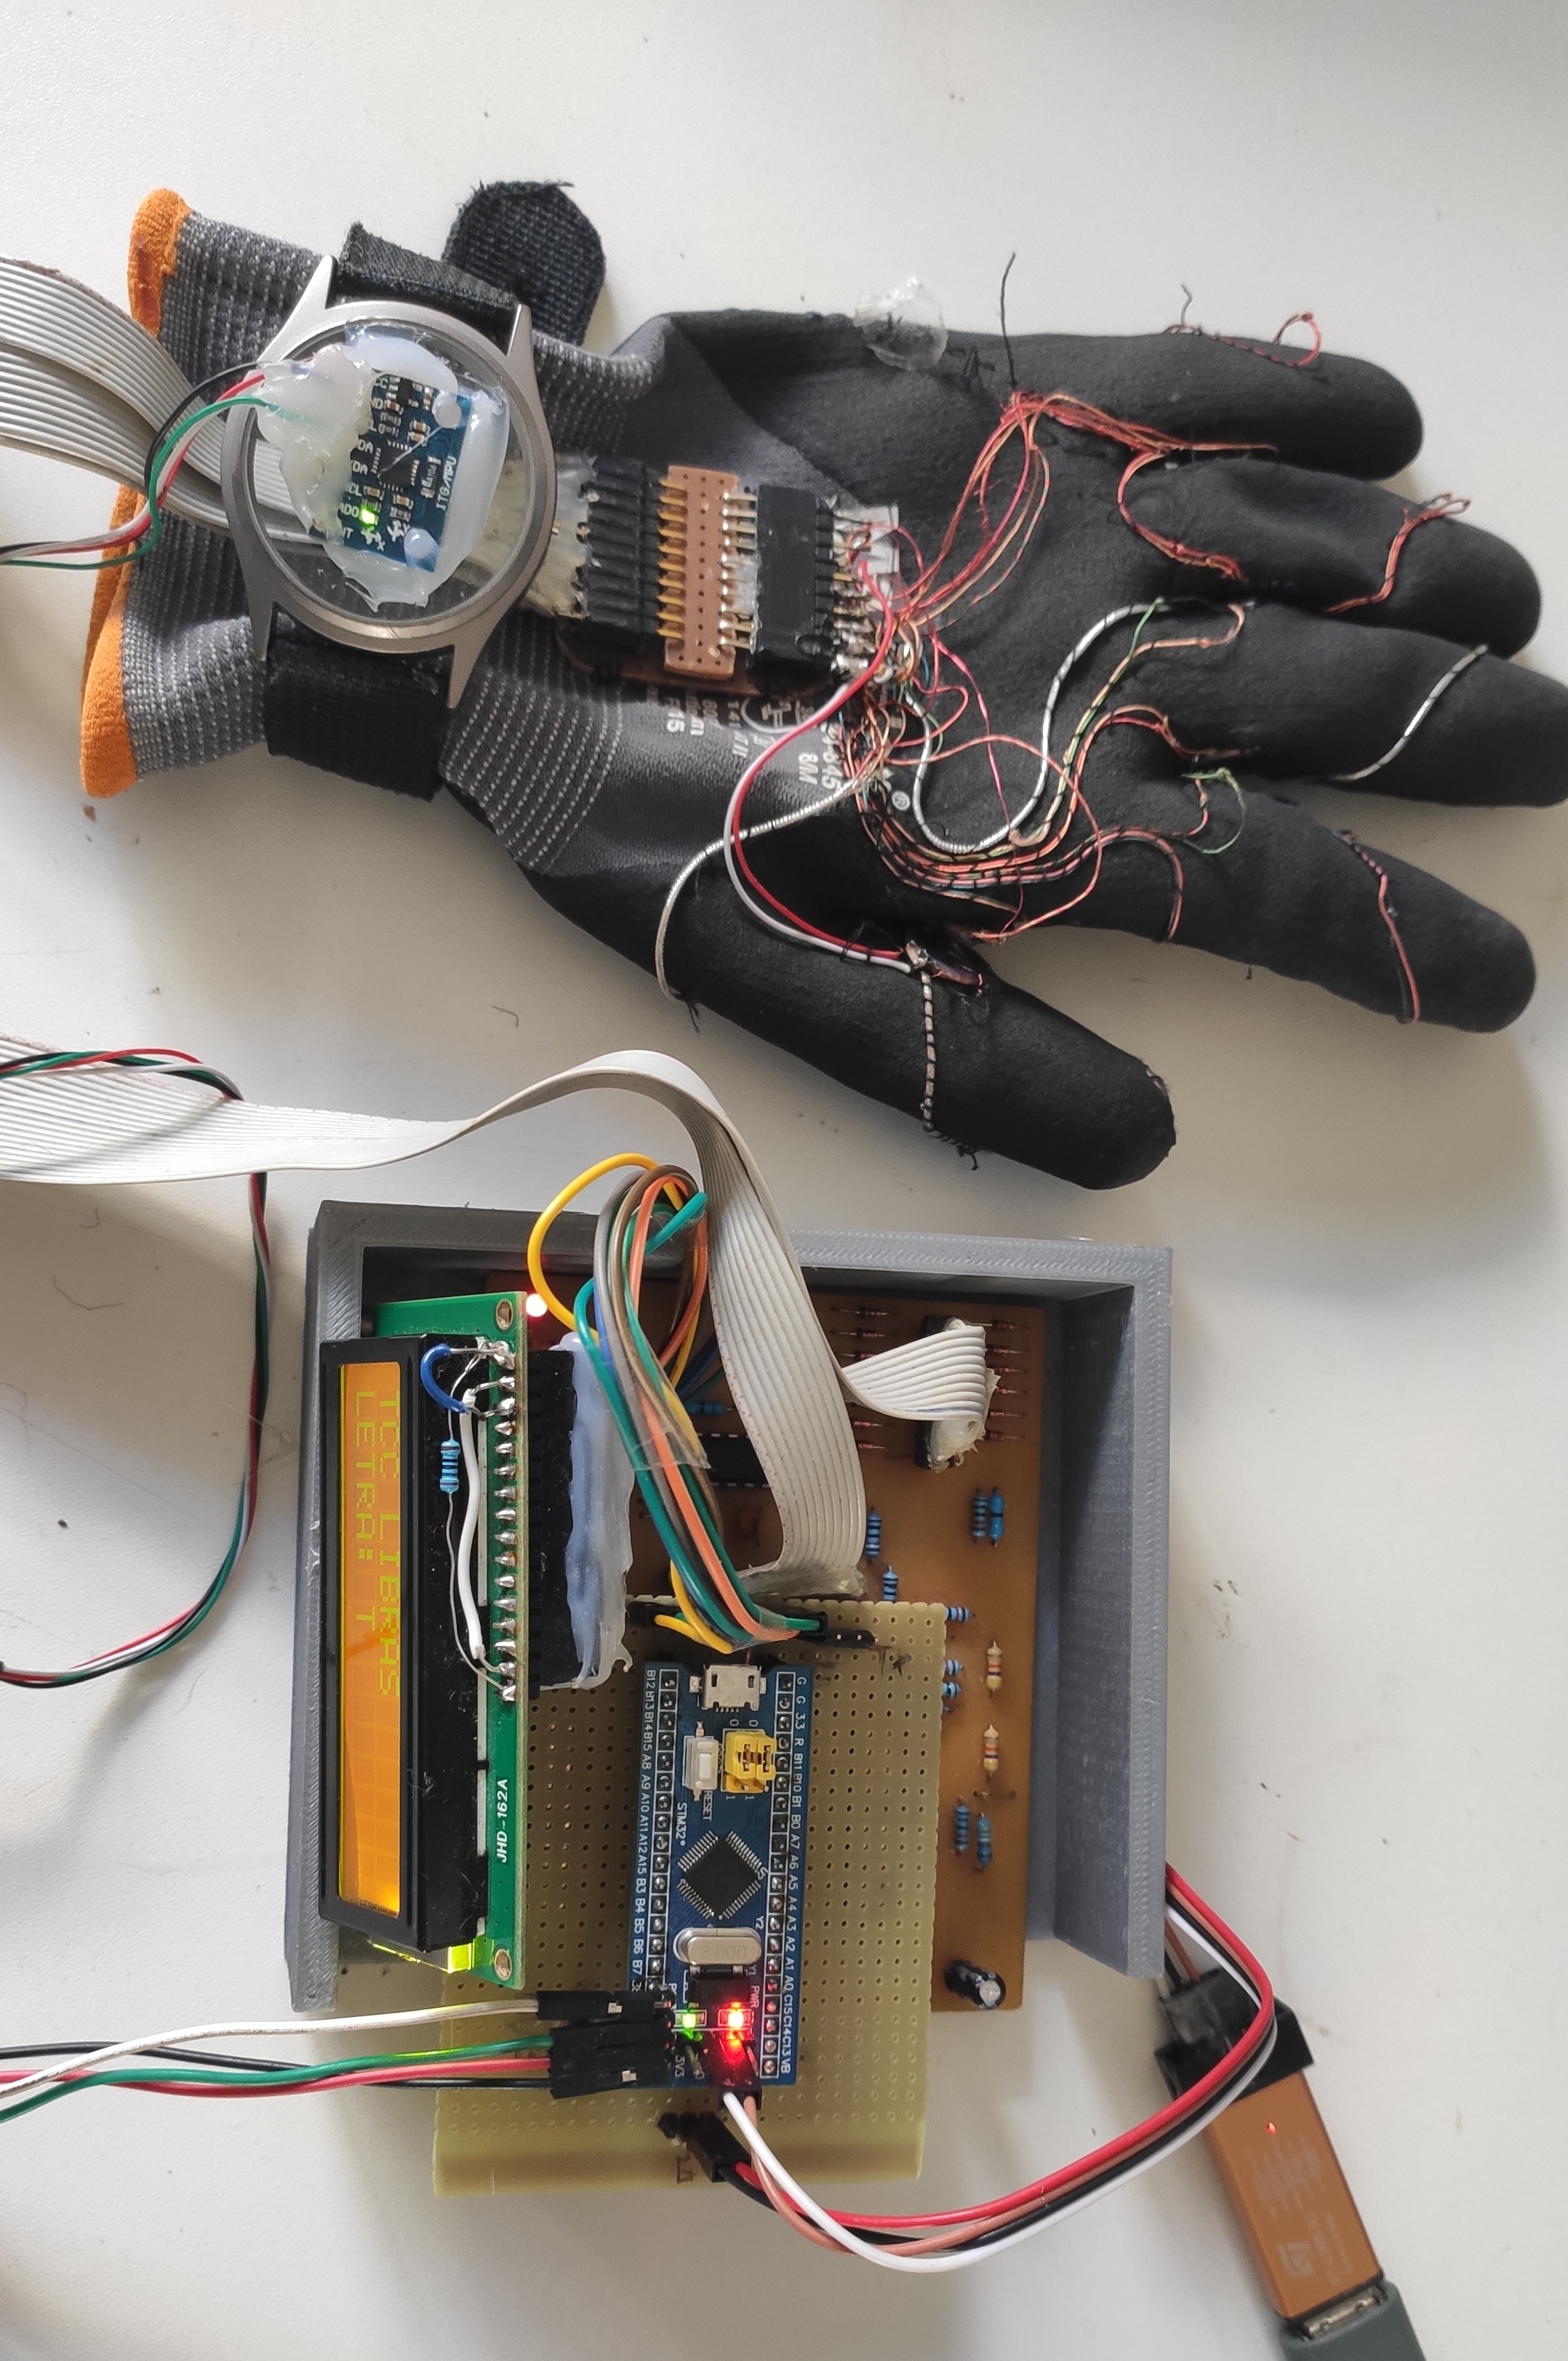
\includegraphics[scale=0.1]{imagens/conjuntoFinal.jpg}
	\caption{Conjunto ao final do trabalho.}
	\label{fig:luvaMontada}
\end{figure}

A Figura \ref{fig:letraC} apresenta uma demonstração da luva formando a letra C e também o \textit{display} mostrando a classificação correta da letra.

\begin{figure}[H]
	\centering
	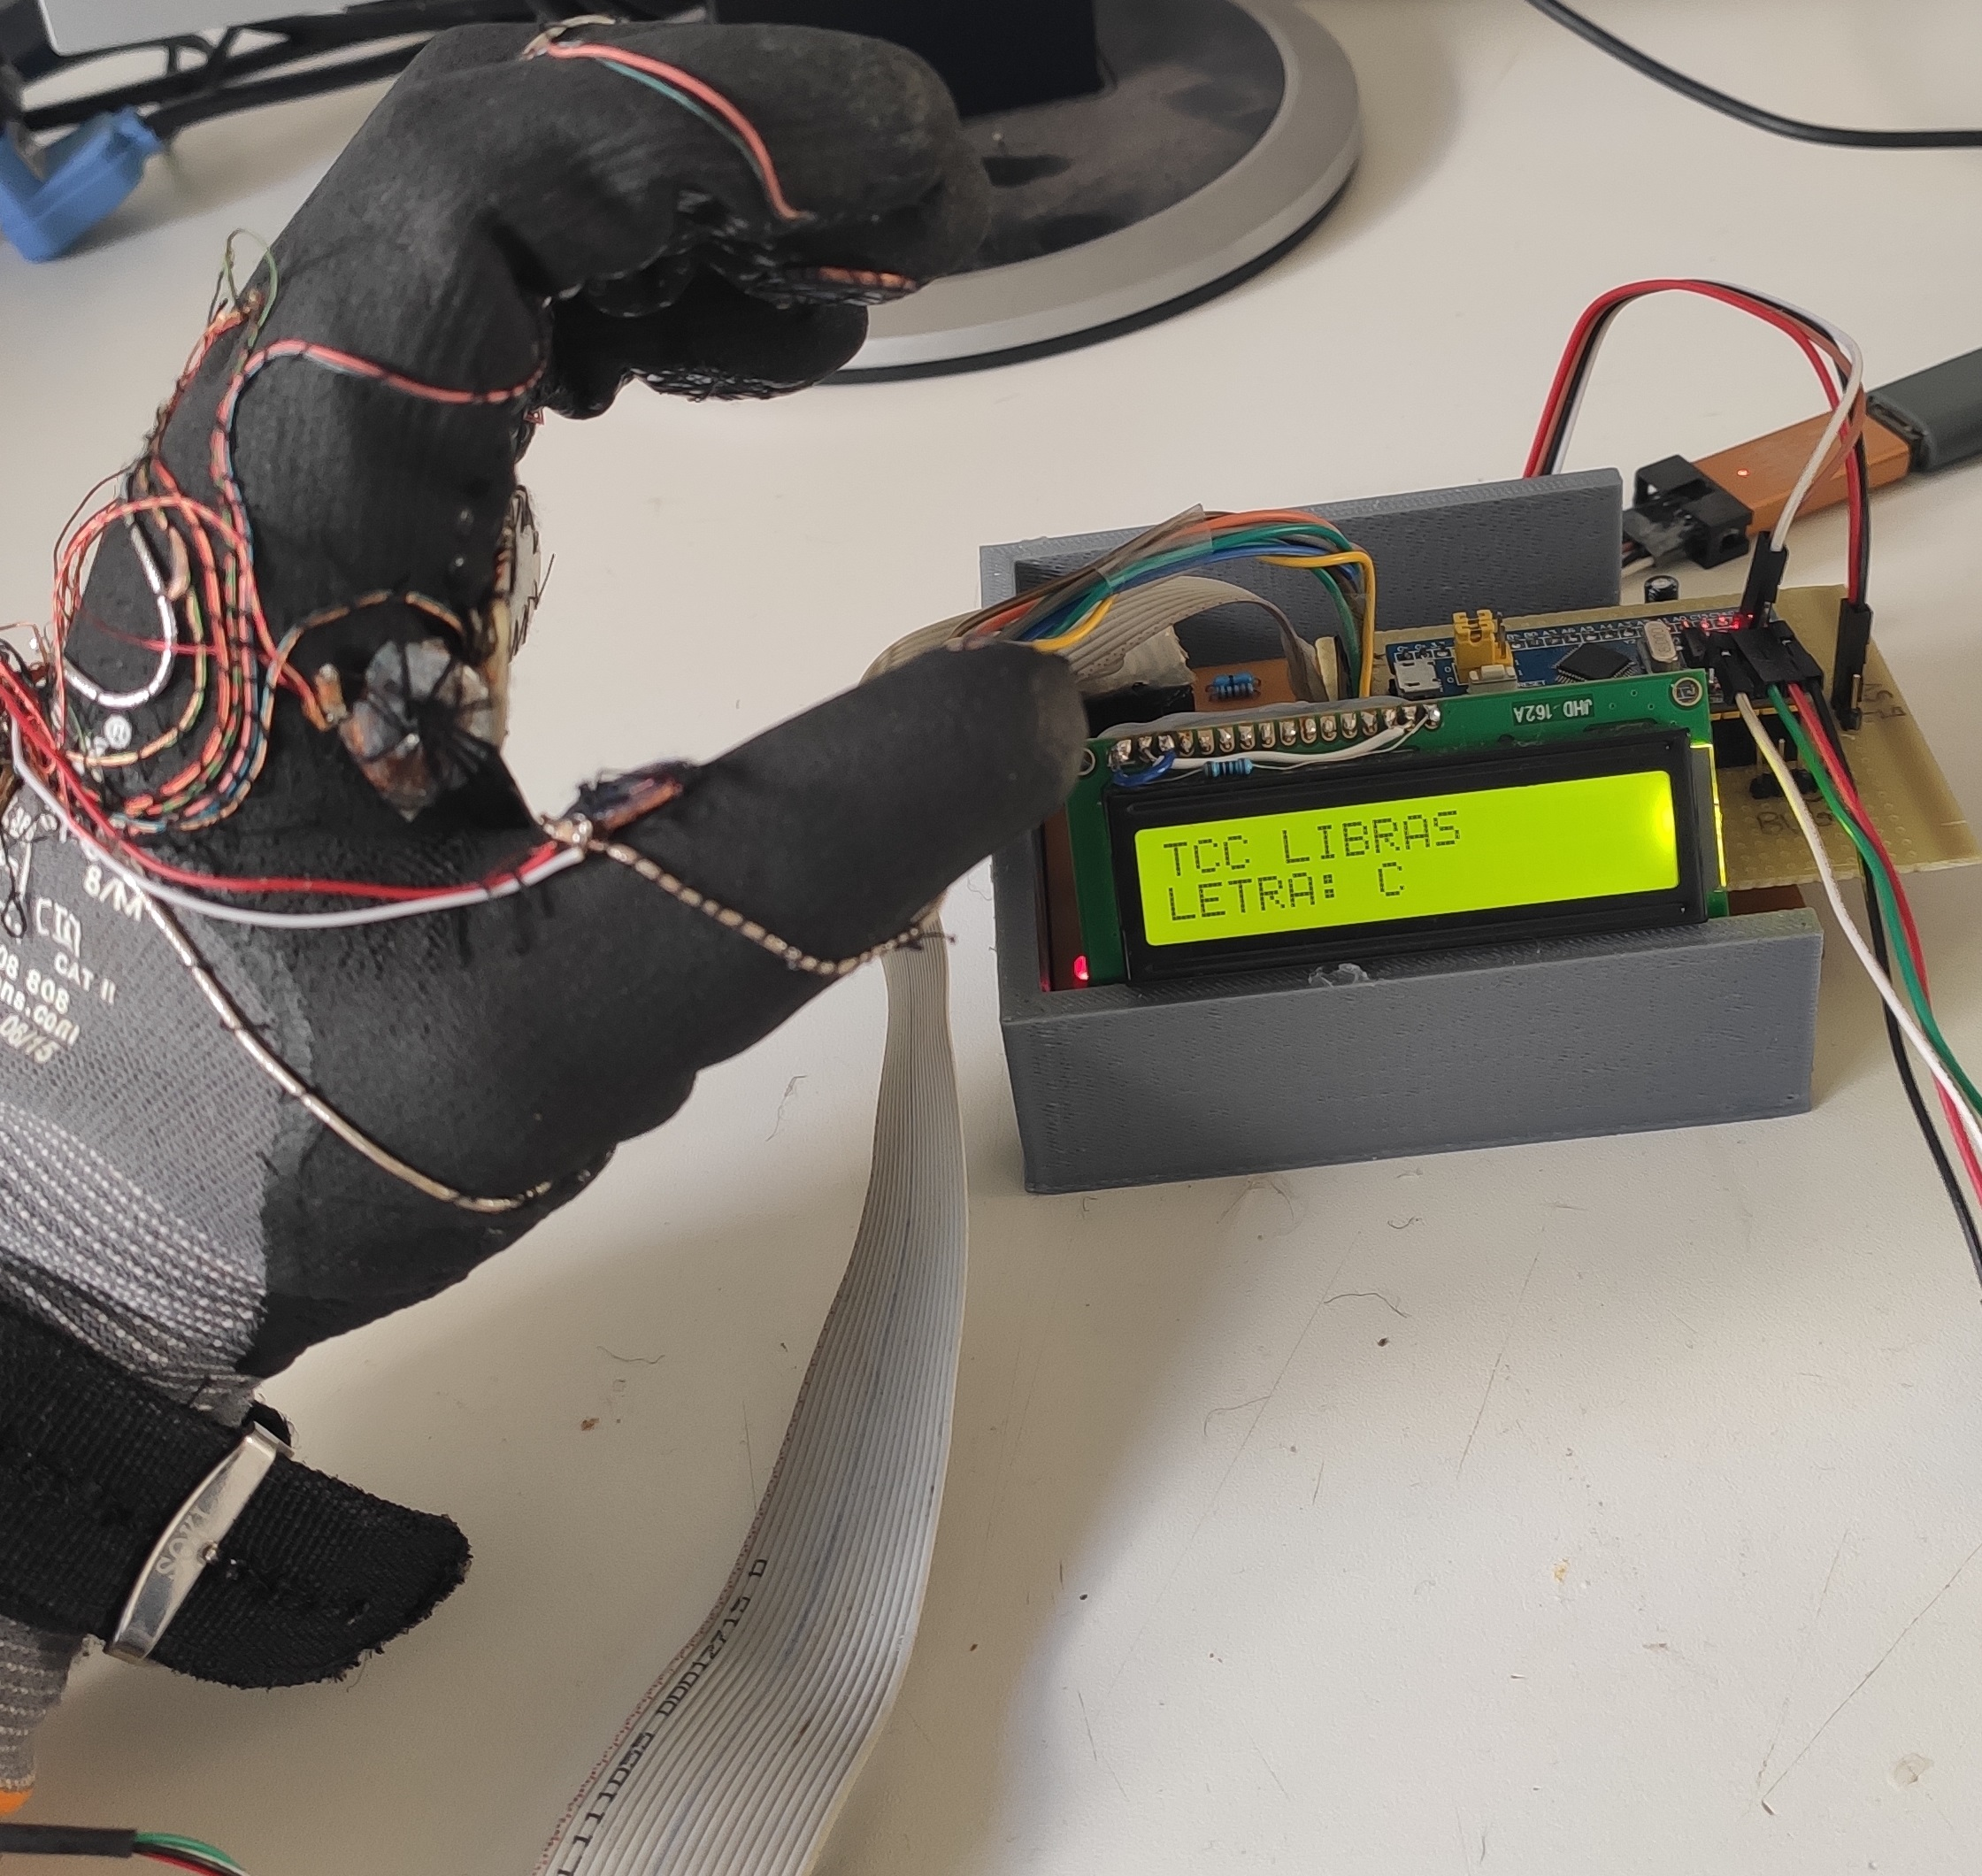
\includegraphics[scale=0.15]{imagens/LetraCLuva.jpg}
	\caption{Demonstração da letra C.}
	\label{fig:letraC}
\end{figure}



 Esse grupo de letras já era classificado no trabalho anterior, mas como a rede foi refeita, ela deve ser validada. Na Tabela \ref{tab:confusaosemconf}, está a matriz de confusão dessa rede refeita, onde foram testada cada letra dez vezes em sequência aleatória.

\begin{table}[H]
	\centering
	\resizebox{\textwidth}{!}{%
		\begin{tabular}{cl|l|l|l|l|l|l|l|l|l|l|l|l|l|l|l|l|l|l|l|}
			\cline{3-21}
			\multicolumn{1}{l}{} &  & \multicolumn{19}{c|}{Classe Predita} \\ \cline{3-21} 
			\multicolumn{1}{l}{} & \textbf{} & \textbf{A} & \textbf{B} & \textbf{C} & \textbf{D} & \textbf{E} & \textbf{F} & \textbf{G} & \textbf{L} & \textbf{M} & \textbf{N} & \textbf{O} & \textbf{Q} & \textbf{R} & \textbf{S} & \textbf{T} & \textbf{U} & \textbf{V} & \textbf{W} & \textbf{Y} \\ \hline
			\multicolumn{1}{|c|}{\multirow{19}{*}{\begin{tabular}[c]{@{}c@{}}C\\ l\\ a\\ s\\ s\\ e\\ \\ R\\ e\\ a\\ l\end{tabular}}} & \textbf{A} & 15 &  &  &  &  &  &  &  &  &  &  &  &  &  &  &  &  &  &  \\ \cline{2-21} 
			\multicolumn{1}{|c|}{} & \textbf{B} &  & 13 & 2 &  &  &  &  &  &  &  &  &  &  &  &  &  &  & \multicolumn{1}{c|}{} &  \\ \cline{2-21} 
			\multicolumn{1}{|c|}{} & \textbf{C} &  &  & 15 &  &  &  &  &  &  &  &  &  &  &  &  &  &  &  &  \\ \cline{2-21} 
			\multicolumn{1}{|c|}{} & \textbf{D} &  &  & 2 & 13 &  &  &  &  &  &  &  &  &  &  &  &  &  &  &  \\ \cline{2-21} 
			\multicolumn{1}{|c|}{} & \textbf{E} &  &  &  &  & 12 &  &  &  &  &  &  &  &  & 3 &  &  &  &  &  \\ \cline{2-21} 
			\multicolumn{1}{|c|}{} & \textbf{F} &  &  &  &  &  & 15 &  &  &  &  &  &  &  &  &  &  &  &  &  \\ \cline{2-21} 
			\multicolumn{1}{|c|}{} & \textbf{G} &  &  &  &  &  &  & 14 & 1 &  &  &  &  &  &  &  &  &  &  &  \\ \cline{2-21} 
			\multicolumn{1}{|c|}{} & \textbf{L} &  &  &  &  &  &  &  & 13 &  &  &  &  &  & 2 &  &  &  &  &  \\ \cline{2-21} 
			\multicolumn{1}{|c|}{} & \textbf{M} &  & 2 &  &  &  &  &  &  & 13 &  &  &  &  &  &  &  &  &  &  \\ \cline{2-21} 
			\multicolumn{1}{|c|}{} & \textbf{N} &  &  &  &  &  &  &  &  &  & 15 &  &  &  &  &  &  &  &  &  \\ \cline{2-21} 
			\multicolumn{1}{|c|}{} & \textbf{O} &  &  &  &  &  &  &  &  &  &  & 15 &  &  &  &  &  &  &  &  \\ \cline{2-21} 
			\multicolumn{1}{|c|}{} & \textbf{Q} &  &  &  &  &  &  &  &  &  &  &  & 13 &  & 2 &  &  &  &  &  \\ \cline{2-21} 
			\multicolumn{1}{|c|}{} & \textbf{R} &  &  &  &  &  &  &  &  &  &  &  &  & 15 &  &  &  &  &  &  \\ \cline{2-21} 
			\multicolumn{1}{|c|}{} & \textbf{S} &  &  &  &  &  &  &  &  &  &  &  &  &  & 15 &  &  &  &  &  \\ \cline{2-21} 
			\multicolumn{1}{|c|}{} & \textbf{T} &  &  &  &  &  &  &  &  &  &  &  &  &  &  & 15 &  &  &  &  \\ \cline{2-21} 
			\multicolumn{1}{|c|}{} & \textbf{U} &  &  &  &  &  &  &  &  &  &  &  &  & 3 &  &  & 12 &  &  &  \\ \cline{2-21} 
			\multicolumn{1}{|c|}{} & \textbf{V} &  &  &  &  &  &  &  &  &  &  &  &  &  &  &  & 1 & 14 &  &  \\ \cline{2-21} 
			\multicolumn{1}{|c|}{} & \textbf{W} &  &  &  &  &  &  &  &  &  &  &  &  &  &  &  &  & 2 & 13 &  \\ \cline{2-21} 
			\multicolumn{1}{|c|}{} & \textbf{Y} & 1 &  &  &  &  &  &  &  &  &  &  &  &  &  &  &  &  &  & 14 \\ \hline
		\end{tabular}%
	}
	\caption{Matriz de confusão das letras sem conflito}
	\label{tab:confusaosemconf}
\end{table}

Contanto todos os erros obtidos da Tabela \ref{tab:confusaosemconf}, temos um total de 21 vezes que uma classe foi classificadas erroneamente. Obtendo um total de 92,63\% de acerto, muito próximo dos 96,36\% de resultado do treinamento.


Agora para as letras conflitantes, como já explicado, a rede neural feita para classificar os movimentos obteve os resultados demonstrados pela Tabela \ref{tab:confusaoconf}.
\begin{table}[H]
	\centering
	\begin{tabular}{cc|c|c|c|c|c|c|c|}
		\cline{3-9}
		&  & \multicolumn{7}{c|}{Classe Predita} \\ \cline{3-9} 
		& \textbf{} & \textbf{I} & \textbf{J} & \textbf{K} & \textbf{H} & \textbf{P} & \textbf{Z} & \textbf{X} \\ \hline
		\multicolumn{1}{|c|}{\multirow{7}{*}{\begin{tabular}[c]{@{}c@{}}R\\ e\\ a\\ l\end{tabular}}} & \textbf{I} & 15 &  &  &  &  &  &  \\ \cline{2-9} 
		\multicolumn{1}{|c|}{} & \textbf{J} & 3 & 10 & 2 &  &  &  &  \\ \cline{2-9} 
		\multicolumn{1}{|c|}{} & \textbf{K} &  &  & 12 &  & 3 &  &  \\ \cline{2-9} 
		\multicolumn{1}{|c|}{} & \textbf{H} &  &  &  & 13 & 2 &  &  \\ \cline{2-9} 
		\multicolumn{1}{|c|}{} & \textbf{P} &  &  &  &  & 15 &  &  \\ \cline{2-9} 
		\multicolumn{1}{|c|}{} & \textbf{Z} &  &  &  &  &  & 15 &  \\ \cline{2-9} 
		\multicolumn{1}{|c|}{} & \textbf{X} &  &  &  &  &  & 6 & 9 \\ \hline
	\end{tabular}
	\caption{Matriz de confusão das letras conflitantes}
	\label{tab:confusaoconf}
\end{table}

Considerando a matriz das letras conflitantes da Tabela \ref{tab:confusaoconf}, temos 88,7\% de acerto, um percentual bom comparado aos 100\% aos do resultado do treinamento no código em Python.

Reunindo o resultado das duas redes, tem-se um percentual de 88,7\% de acerto. Esses 11,3 \% de erro são justificados por vários fatores. Um deles são os pontos cegos dos sensores indutivos como \citeonline{RUANI} descreve nos em seus resultados que podem ser resolvidos modificando a posição dos sensores e adicionando mais sensores indutivos. Também se deve ao fato de se estar utilizando somente o acelerômetro na classificação, onde poderia obter maior precisão utilizando giroscópio. A abordagem de janela deslizante funcionou bem, mas para uma classificação mais efetiva seria necessário uma abordagem de um algoritmo de aprendizagem de máquina que considera o tempo para aumentar essa taxa de acerto.
